%------------------------------------------------------
%Author             : Daniel Schembri, Jonathan Schwarz
%University         : Pforzheim University
%Date of last edit  : Wed, 03 Sep 2014 14:12:16 +0200
%Filename           : multithreading_with_posix_pthreads.tex
%------------------------------------------------------

\documentclass[10pt,a4paper,DIV=11]{scrreprt}

%British English
\usepackage[UKenglish]{babel}
%utf8
\usepackage[utf8]{inputenc}

%pseudo-code
\usepackage[boxruled,vlined]{algorithm2e}

%for source code listings
\usepackage{listings}

\usepackage[table]{xcolor}

%tikz
\usepackage{tikz}
\usetikzlibrary{arrows,positioning,fit}

%plots
\usepackage{pgfplots}

%blocks - used by tikz-uml, included before
\pgfdeclarelayer{background}
\pgfdeclarelayer{foreground}
\pgfsetlayers{background,main,foreground}

%<,> in tikz-uml
\usepackage[T1]{fontenc}
\usepackage{tikz-uml}

%subfigure
\usepackage{graphicx}
\usepackage{subfigure}

%prevent figure from floating pictures
\usepackage{float}

%footer & header
\usepackage{fancyhdr}

%push footer down
\usepackage[bottom]{footmisc}

%footer & header
\pagestyle{fancy}
%clean footer & header
\fancyhf{}

%bibtex
\usepackage[square,numbers]{natbib}
\usepackage{gensymb}

%equation
\usepackage[tbtags]{amsmath}
\usepackage{amssymb} 

%table of contents with hyperlinks
%always include as last package
\usepackage{hyperref}

%===========================TITLE PAGE=======================================

%university logo
\titlehead
{
    
\includegraphics[width=0.20\textwidth]{files/hspflogo.pdf}\\

    Pforzheim University\\
    School of Engineering\\
}

\subject{Project work}
	
\title
{
    Simulation and evolutionary training of object collectiong agents (STOCA)\\
}

\author
{
    by \textbf{Daniel Schembri} - matriculation number: 310026
}
\date
{
    Winter term 2013/2014
}
%\today{}}

\publishers
{
    Examiner: Prof. Dr. Richard Alznauer\\
    Supervisor: Dr. Christoph Ussfeller
}


%=========================================GLOBAL SETTINGS=========================================

%footer &header

%\fancyfoot[L]{\textbf{Multi-Threading mit POSIX-pThreads}}
\fancyhead[R]{Page \thepage}
%\fancyhead[L]{\thechapter}

%chapter number and title
\fancyhead[L]{\nouppercase{\leftmark}}
%line
%\renewcommand{\footrulewidth}{0.5 pt}
\usepackage{lmodern}
\addtokomafont{sectioning}{\rmfamily}
\setlength{\parindent}{0mm}

%colour definitions
\definecolor{dkgreen}{rgb}{0,0.6,0}
\definecolor{gray}{rgb}{0.7,0.7,0.7}
%medium gray
\definecolor{mgray}{gray}{0.80}
%light gray
\definecolor{lgray}{gray}{0.97}

%hyperlink settings
%frame around hyperlinks
\hypersetup
{
    colorlinks = false,
    linkcolor = black,
    hypertexnames = false,
    citecolor = green
}

%listing settings
\lstset
{ 
    language=C,                
    basicstyle=\footnotesize\ttfamily,           
    numbers=left,
    stepnumber=5,    
    firstnumber=1,
    numberfirstline=true                 
    numberstyle=\color{black},                 
    numbersep=5pt,                 
    backgroundcolor=\color{white},      
    showspaces=false,             
    showstringspaces=false,         
    showtabs=false,                
    frame=single,                   
    rulecolor=\color{black},       
    tabsize=2,                     
    captionpos=b,                   
    breaklines=true,                
    breakatwhitespace=false,       
    title=\lstname,                    
    keywordstyle=\color{blue},          
    commentstyle=\color{dkgreen}, 
    identifierstyle=\color{black},      
    stringstyle=\color{purple},      
    escapeinside={\%*}{*)},      
    morekeywords={*,...},            
    deletekeywords={...}             
}

\setcounter{tocdepth}{4}  %a deeper contentsmenue
%=====================================DOCUMENT START=========================
\begin{document}

\tikzstyle{line}=[draw]
\tikzstyle{arrow}=[draw, -latex] 

%\renewcommand*\contentsname{Content}
%\renewcommand*\listtablename{Tables}
%\renewcommand*\listfigurename{Figures}
%\renewcommand*\bibname{Literature references}

\maketitle
\thispagestyle{empty}
\newpage
{\large\tableofcontents}
\newpage

% Ideas for the documentation 
% -> Robots playing football
% -> 
% 
%
%
%
%



\chapter{Introduction}
Intelligent systems are widely used, like in robotics.
The motivation to write this projectwork was
to find out basically, how an intelligent system can be created by simple algorithms (rules) and compare them with 'classical' solutions. Therefore a simple task was to let agents collect objects in a virtual environment.



In this project neural networks of the second type are used, because the main interest lies in finding a good mathematical solution.



\section{State of the art}

\section{Artificial intelligence}
Today there is not a definition of what intelligence exactly is.
In general there certain categories focusing parts to describe of
intelligents.

\subsection{}


\subsection{The concept of agents}
An agent is a programm that interacts self-sufficent depending on the actual state. It has sensors, a processing logic and actuators to interact with its environment. The input data will be processed to behave in the desired way. In the simplest case this could be a table containing the required output to every possible input. In this project the 



\begin{center}
	\begin{figure}[H]
		\centering
		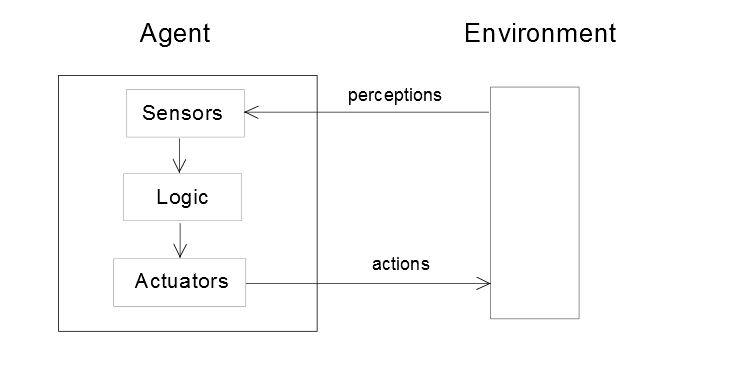
\includegraphics[width=1.0\textwidth,scale=1]{files/agent.png}  
		\caption{Structure of an agent (oriented on \cite{ki-book} )} 
		\label{fig:agent}
	\end{figure}
\end{center}

\subsection{Basics of artificial neural networks}

\section{Applications}

\chapter{Optimization with evolutionary algorithms}
Optimization is widely used, for example in information technology, engineering,
economics, etc. Applications are the routing of circuits, the optimal usage of machinery,
the traveling-salesman-problem and much more. It is often difficult to create a mathematical
model of such optimization problems. Therefore in the last decades were developed methods who
uses principles of the evolution.
The simples method is the selection-method. In this model a dateset will be generated and randomly
changes, called mutations, are made. The best datasets, chosen by the best fitness, will be kept.
Each dateset is called an individual. A set of individuals is called a population. The individuals
of a population can be recombined. Mostly the best individuals are recombined with randomly chosen
ones. This method is more effective than the selection-method. This and other methods are  called
evolutionary algorithms. To use an evolutionary algorithm, the problem must not be in a defined form;
therefore it hasn't to be linear or differentiable. \\

In this project evolutionary algortihms are used to find the best 
(unsupervised) neural network to controll one creature. The idea is to use the amount of food a creature collect over a defined time as fitnessvalue.

\section{The creepy random search method or hill climber method}
The creepy random search method is a basic method of an evolutionary algorithm, developed by Ingo Rechenberg in 1973. % 1973 correct?? look at literaturesource in kinnebruck
Parameters of a system are randomly changed till a minimum or maximum of a targetfunction is reached. The value of the parameterchanges per iterationstep are limited. \\

\textbf{The main algorithm is:}

\fbox{
	\begin{minipage}{15cm}
		\begin{enumerate} 
			\item Generate a randomly initialized chromosome.
			\item Change the chromosome parameter by limited random delta-values. 
			\item Prove if the chromosome has a better fitness than the old one and replace it. Otherwise forget the new chromosome.
			\item If the optimization-condition is reached abort, otherwise go to step 2.
		\end{enumerate}
	\end{minipage}
} \\

The algorihm can be imagined as a blind hillclimber. The hillclimber makes a random step. If he gets higher, he makes the next step. Otherwise he takes back his last step and makes another random step. The big problem is, that this algorithm mostly converges in a local optimum. \\

\textbf{Reasons to use this kind of algorithm:}

\fbox{
	\begin{minipage}{15cm}
		\begin{itemize} 
			\item For many nonlinear problems there are no alternative solution approaches.
			\item Implementing this method is easy.
		\end{itemize}
	\end{minipage}
}   \\



\begin{center}
	\begin{figure}[H]
		\centering
		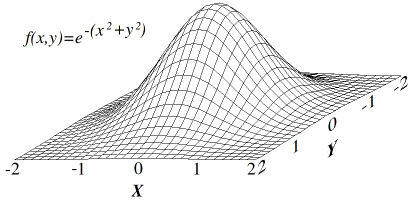
\includegraphics[width=0.6\textwidth,scale=1]{files/Hill_climb.png}  
		\caption{A convex function. Ideal for the hillclimbing method \cite{wiki-hill}.}
		\label{fig:hill}
	\end{figure}
\end{center}

\begin{center}
	\begin{figure}[H]
		\centering
		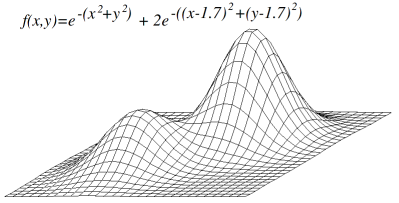
\includegraphics[width=0.6\textwidth,scale=1]{files/Local_maximum.png}  
		\caption{A function with two optima. Hillclimbing could end in the worse optimum if it starts at a bad coordinate. \cite{wiki-hill}.}
		\label{fig:hill2}
	\end{figure}
\end{center}


\subsection{Constraints} %Bedingungen und Nebenbedingungen
The main condition is the fitness-function. Second conditions
can be the

%\subsection{Efficency} %Optional chapter to test the efficency between mathematical methods and evolutionary methods. For example zero of a function.

\section{Variants of the creepy random search method}
In the main-method of the creepy random search you just accept better fitness values after an iteration-step and reject worse ones.
The problem is, that with this algorithm you will mostly get stuck on a local optimum, instead of finding the global one.
To solve this problem you should allow temporal low fitness-values. It should be possible to leave a local optimum to find a better one.
To realise this, there have been developed some extended versions of this method: \\

\fbox{
	\begin{minipage}{15cm}
		\begin{itemize} 
			\item A stagnation of the fitness is allowed by a specified probability (Simulated annealing)
			\item A stagnation of the fitness is allowed till a maximal deterioration. (Threshold accepting, deluge method)
		\end{itemize}
	\end{minipage}
} \\


\subsection{Simulated annealing}
Simulated annealing is a probabilistic optimization method.
It is inspired by the annealing of fluid materia to a solid aggregate states in metallurgy. While cooling down a material the thermodynamic free energy has to get as minimal as possible to get a clear crystalline structure. Therefore its suggested to cool down to material slowly for a better probability of getting a clear solid body.

Analog in optimization you start with a high temperature T, means a big delta, to make wide jumps in the problemphase-space. So jumps between more maxima are possible. At the beginning each chromosome has the same probability to get selected. With each iteration the temperature is reduced and the jumps are getting shorter. Selecting better chromosomes is now more probalistic.
Towards the end the algorithm commutes in a optimum and behaves like the standard hillclimbing-algorithm.

Slowly reducing the temperature increases the chance to find the global optimum. Cooling to fast leads to commuting early into a local optimum instead.

The following formula shows the probability of selecting a chromosome with lower fitness:

\begin{equation}
p(r) = \frac{1}{1+exp(-r/T)}
\end{equation} 

The probability to select a worse chromosome should be small.
At the beginning a big T tends to equalize the probability of all chromosomes. For $T \to \infty$ all chromosomes have the same chance to get selected. Lowering T gives good chromosomes priority. For T = 0.1

\subsection{Threshold accepting}

\section{Applications}

% \section{Genetic algorithms - An artifical duck}

\chapter{Alternative algorithms}
In this chapter other intelligent algorithms are presented.
These algortihms are for comparing the neural network to simpler
methods.

\section{The greedy algorithm}

\subsection{Weaknesses}

\section{Applications}





\chapter{Development of a simulator for virtual agents}

\section{Concept}


Transformation of the inputvalues through the input-neurons from range [-20.0, 20.0] and [0.0, 20.0] (Sensor x and y) and [-Pi, +Pi] (DeltaAngle) to the range [-1.0,+1.0] or [0.0, 1.0] with tanh function. (Better function? Linear function?)

Explain why DeltaAngle is necessary:
rotate clockwise. If Agent is rotated by 180degree error should rotate counter-clockwise,but
has learned to rotate clockwise without deltaangle as input.


Optional: Random placment of Objects and agents: see algorithm in NeuralWorld.cpp



Scalability of the World


Modes:
Singleplayer with recording
Supervised learning:
Evolutionary algorithms

Scalable World:
- Size
- Amount of Objects
- Amount of Agents

\section{Software-Engineering}

\subsection{Classdiagram}

\subsection{Use-Cases}

\subsection{The graphical user interface}

Buttons, Modes

Weight-Matrix

Neural Network Activation

\subsection{The interface}


The inputs: 
x  [0.0, 20.0]
y   [0.0, 20.0]
alpha  [-PI, PI] (Radians)

If no object is detected :
x = 0
y = 0,
alpha = 0 

If an object is detected:
x= Agent.x - Object.x  
y = Agent.y - Object.y
alpha = Agent.Angle - (atan2(det, dot)) 
alpha is the difference between the actual direction of the agent and
the angle between the Position vector of the agent and the object. 
Helpervariables:
determinant: det =  Agent.x * Object.y - Agent.y * Object.x 
dot product:  dot =  Agent.x * Object.x + Agent.y * Object.y 


Outputs are:
Acceleration of the agent: [0.0, 1.0] (with a resolution of 0.001)
multiplied with the maximum accelartion of 
(-sin(Agent->GetAngle())*0.075f * 500 * ,  cos(Agent->GetAngle())*0.075f * 500)

Rotation by angle the agent: [-1.0, 1.0] (with a resolution of 0.001)
multiplied with the maximum rotationspeed of 0.075


%The
%To minimize  that the agents are missing

\section{OpenGL}

GLUT, Windows Substitute Freeglut and GLUI. (used because Box2D Testbed used it)


\section{The Box2D-Physicsengine}

    AnimalFixtureDef[i].isSensor = false;
    AnimalFixtureDef[i].friction = 1.0f;
    AnimalBodydef[i].linearDamping = 1.0f;
    AnimalBodydef[i].angularDamping = 2.0f;

\section{Tools}
Make, CMake
Python for Trainingdata

\section{Visualisation}

Fitness Graph
Weight Matrix
Neural Network
% \subsection{The fitness-function}


% \subsection{Neural networks}

\chapter{Results of the simulation}

\chapter{Conclusion}




\KOMAoptions{listof=leveldown}

\newpage

%=========================================LISTS=========================================

\listoffigures
\listoftables
\listofalgorithms
\lstlistoflistings

\newpage

%=========================================DICTIONARY====================================

%dictiary style
\bibliographystyle{./files/alphadin}
%dictionary source
\bibliography{./files/bibdb}


%AI-Junkie Smart Sweepers

%Evolutionäre Algorithmen
%Theorie der neuronalen Netze
%Jonathan Schwarz
%Künstliche Intelligenz

%Box2D Manual
%Box2D Iforce2D

%CMake Manual
%Makefile Manual

%Software-Engineering books?

%Opengl, GLUT and GLUI



\end{document}
